\section{Experiments}

% \begin{frame}{Outline}
% \tableofcontents[currentsection]
% \end{frame}

\begin{frame}{Experimental Setup}

\begin{columns}
\column{0.4\textwidth}
Image classification datasets:
\begin{itemize}
    \item SVHN (10-way)
    \item CIFAR-10 (10-way)
    \item CIFAR-100 (100-way)
\end{itemize}

\column{0.6\textwidth}

Model architectures:
\begin{itemize}
    \item PreActResNet18 (He \etal, 2016)
    \item VGG16 (Simonyan \etal, 2015)
    \item WideResNet-28-10 (Zagoruyko \etal, 2016)
    \item PyramidNet-164-270 (Han \etal, 2017)
\end{itemize}
\end{columns}

\begin{columns}
\column{0.7\textwidth}
Compared methods:
\begin{itemize}
    \item ERM (Vapnik \etal, 1998)
    \item Dropout (Srivastava \etal, 2014)
    \item Label smoothing (Szegedy \etal, 2016)
    \item Flooding (Ishida \etal, 2020)
    \item MixUp (Zhang \etal, 2018)
    \item Adversarial Training (Goodfellow \etal, 2015)
\end{itemize}
\column{0.3\textwidth}
\end{columns}

\vspace{1.5em}

\end{frame}


\begin{frame}{Loss Curves}

\begin{figure}
\subcaptionbox{CIFAR-10 Training Set}[.48\textwidth]{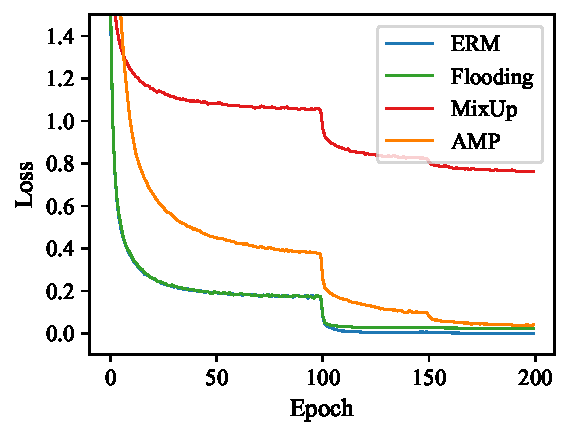
\includegraphics[width=.45\textwidth]{figs/cifar10_preactresnet18_train_loss.pdf}}
\subcaptionbox{CIFAR-10 Test Set}[.48\textwidth]{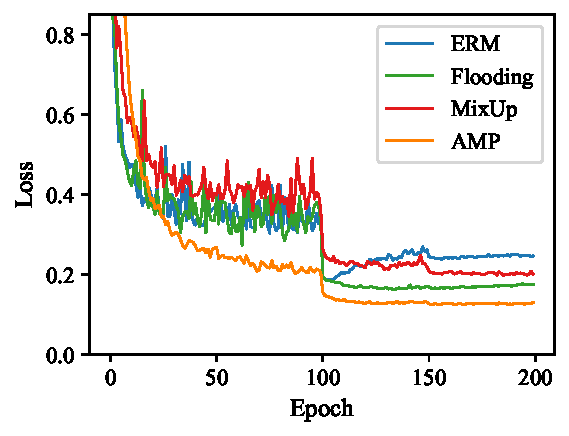
\includegraphics[width=.45\textwidth]{figs/cifar10_preactresnet18_test_loss.pdf}}
\end{figure}

\end{frame}

\begin{frame}{Results on Image Classification Benchmarks}

\begin{table}[t]
\centering
\subcaptionbox{SVHN\label{tab:svhn}}[.33\textwidth]{%
\resizebox{.33\textwidth}{!}{%
\begin{tabular}{lcc}
\toprule
PreActResNet18 & Test Error (\%) & Test NLL \\
\midrule
ERM & 2.95$\pm$0.063 & 0.166$\pm$0.004 \\
Dropout & 2.80$\pm$0.065 & 0.156$\pm$0.012 \\
Label Smoothing & 2.78$\pm$0.087 & 0.998$\pm$0.002 \\
Flooding & 2.84$\pm$0.047 & \underline{0.130$\pm$0.003} \\
MixUp & \underline{2.74$\pm$0.044} & 0.146$\pm$0.004 \\
Adv. Training & 2.77$\pm$0.080 & 0.151$\pm$0.018 \\
RMP & 2.93$\pm$0.066 & 0.161$\pm$0.010 \\
AMP & \textbf{2.30$\pm$0.025} & \textbf{0.096$\pm$0.002} \\
\midrule
VGG16 & Test Error (\%) & Test NLL \\
\midrule
ERM & 3.14$\pm$0.060 & 0.140$\pm$0.027 \\
Dropout & 2.96$\pm$0.049 & 0.134$\pm$0.027 \\
Label Smoothing & 3.07$\pm$0.070 & 1.004$\pm$0.002 \\
Flooding & 3.15$\pm$0.085 & 0.128$\pm$0.003 \\
MixUp & 3.09$\pm$0.057 & 0.160$\pm$0.003 \\
Adv. Training & \underline{2.94$\pm$0.091} & \underline{0.122$\pm$0.003} \\
RMP & 3.19$\pm$0.052 & 0.134$\pm$0.004 \\
AMP & \textbf{2.73$\pm$0.015} & \textbf{0.116$\pm$0.006} \\
\bottomrule
\end{tabular}
}%
}%
\subcaptionbox{CIFAR-10\label{tab:cifar10}}[.33\textwidth]{%
\resizebox{.33\textwidth}{!}{%
\begin{tabular}{lcc}
\toprule
PreActResNet18 & Test Error (\%) & Test NLL \\
\midrule
ERM & 5.02$\pm$0.212 & 0.239$\pm$0.009 \\
Dropout & 4.86$\pm$0.148 & 0.223$\pm$0.009 \\
Label Smoothing & 4.85$\pm$0.115 & 1.038$\pm$0.003 \\
Flooding & 4.97$\pm$0.082 & \underline{0.166$\pm$0.003} \\
MixUp & \underline{4.09$\pm$0.117} & 0.198$\pm$0.004 \\
Adv. Training & 4.99$\pm$0.085 & 0.247$\pm$0.006 \\
RMP & 4.97$\pm$0.167 & 0.239$\pm$0.008 \\
AMP & \textbf{3.97$\pm$0.091} & \textbf{0.129$\pm$0.003} \\
\midrule
VGG16 & Test Error (\%) & Test NLL \\
\midrule
ERM & 6.32$\pm$0.193 & 0.361$\pm$0.012 \\
Dropout & 6.22$\pm$0.147 & 0.314$\pm$0.009 \\
Label Smoothing & 6.29$\pm$0.158 & 1.076$\pm$0.003 \\
Flooding & 6.26$\pm$0.145 & \underline{0.234$\pm$0.005} \\
MixUp & \textbf{5.48$\pm$0.112} & 0.251$\pm$0.003 \\
Adv. Training & 6.49$\pm$0.130 & 0.380$\pm$0.010 \\
RMP & 6.30$\pm$0.109 & 0.363$\pm$0.010 \\
AMP & \underline{5.65$\pm$0.147} & \textbf{0.207$\pm$0.005} \\
\bottomrule
\end{tabular}
}%
}%
\subcaptionbox{CIFAR-100\label{tab:cifar100}}[.33\textwidth]{%
\resizebox{.33\textwidth}{!}{%
\begin{tabular}{lcc}
\toprule
PreActResNet18 & Test Error (\%) & Test NLL \\
\midrule
ERM & 24.31$\pm$0.303 & 1.056$\pm$0.013 \\
Dropout & 24.48$\pm$0.351 & 1.110$\pm$0.021 \\
Label Smoothing & 22.07$\pm$0.256 & 2.099$\pm$0.005 \\
Flooding & 24.50$\pm$0.234 & 0.950$\pm$0.011 \\
MixUp & \underline{21.78$\pm$0.210} & \underline{0.910$\pm$0.007} \\
Adv. Training & 25.23$\pm$0.229 & 1.110$\pm$0.012 \\
RMP & 24.28$\pm$0.138 & 1.059$\pm$0.011 \\
AMP & \textbf{21.51$\pm$0.308} & \textbf{0.774$\pm$0.016} \\
\midrule
VGG16 & Test Error (\%) & Test NLL \\
\midrule
ERM & 27.84$\pm$0.297 & 1.827$\pm$0.209 \\
Dropout & 27.72$\pm$0.337 & 1.605$\pm$0.062 \\
Label Smoothing & 27.49$\pm$0.179 & 2.310$\pm$0.005 \\
Flooding & 27.93$\pm$0.271 & 1.221$\pm$0.037 \\
MixUp & \underline{26.81$\pm$0.254} & \underline{1.136$\pm$0.013} \\
Adv. Training & 29.12$\pm$0.145 & 1.535$\pm$0.389 \\
RMP & 27.81$\pm$0.327 & 1.873$\pm$0.035 \\
AMP & \textbf{25.60$\pm$0.168} & \textbf{1.049$\pm$0.049} \\
\bottomrule
\end{tabular}
}%
}%
\caption{Top-1 classification errors and test neg-log-likelihoods.}
\end{table}

\end{frame}

\begin{frame}{Improvement over Data Augmentation}

\begin{table}[t]
\centering
\resizebox{.9\columnwidth}{!}{%
\begin{tabular}{llcccc}
\toprule
 & & \multicolumn{2}{c}{WideResNet-28-10} & \multicolumn{2}{c}{PyramidNet-164-270}\\
 & & ERM & AMP & ERM & AMP \\
\midrule
 & Vanilla & 2.57$\pm$0.067 & \textbf{2.19$\pm$0.036} & 2.47$\pm$0.034 & \textbf{2.11$\pm$0.041} \\
SVHN & Cutout & 2.27$\pm$0.085 & \textbf{1.83$\pm$0.018} & 2.19$\pm$0.021 & \textbf{1.82$\pm$0.023} \\
 & AutoAug & 1.91$\pm$0.059 & \textbf{1.61$\pm$0.024} & 1.80$\pm$0.044 & \textbf{1.35$\pm$0.056} \\
\midrule
 & Vanilla & 3.87$\pm$0.167 & \textbf{3.00$\pm$0.059} & 3.60$\pm$0.197 & \textbf{2.75$\pm$0.040} \\
CIFAR-10 & Cutout & 3.38$\pm$0.081 & \textbf{2.67$\pm$0.043} & 2.83$\pm$0.102 & \textbf{2.27$\pm$0.034} \\
 & AutoAug & 2.78$\pm$0.134 & \textbf{2.32$\pm$0.097} & 2.49$\pm$0.128 & \textbf{1.98$\pm$0.062} \\
\midrule
 & Vanilla & 19.17$\pm$0.270 & \textbf{17.33$\pm$0.110} & 17.13$\pm$0.210 & \textbf{15.09$\pm$0.092} \\
CIFAR-100 & Cutout & 18.12$\pm$0.114 & \textbf{16.04$\pm$0.071} & 16.45$\pm$0.136 & \textbf{14.34$\pm$0.153} \\
 & AutoAug & 17.79$\pm$0.185 & \textbf{14.95$\pm$0.088} & 15.43$\pm$0.269 & \textbf{13.36$\pm$0.245} \\
\bottomrule
\end{tabular}
}
\caption{Top-1 classification errors and test neg-log-likelihoods.}
\end{table}

\end{frame}

\begin{frame}{Calibration Results}

Expected Calibration Error: (lower is better)
\begin{equation*}
\text{ECE}=\sum_{m=1}^M\frac{|B_m|}{n}\bigg\vert\underbrace{\frac{1}{|B_m|}\sum_{i\in B_m}\mathbf{1}(\hat{y}_i=y_i)}_{\text{accuracy}}-\underbrace{\frac{1}{|B_m|}\sum_{i\in B_m}\hat{p}_i}_{\text{confidence}}\bigg\vert
\end{equation*}
\vspace{-0.5em}

\begin{figure}
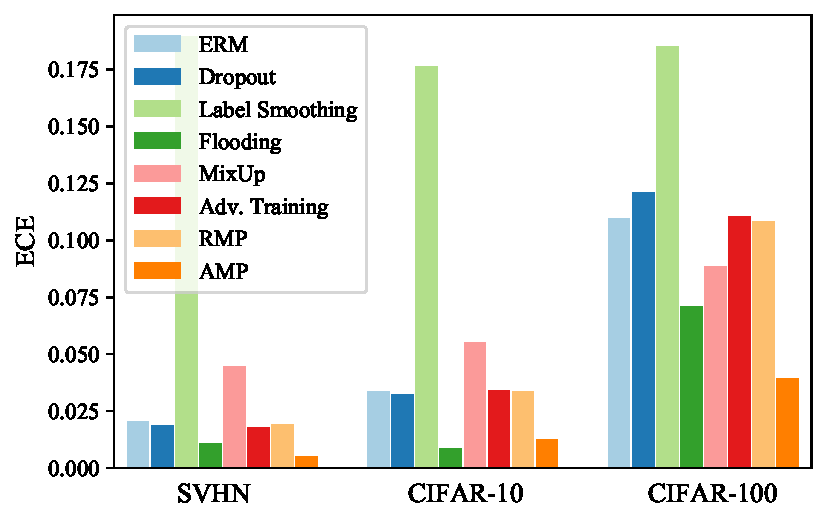
\includegraphics[width=.46\textwidth]{figs/ece.pdf}
\end{figure}

\vspace{1em}

\end{frame}

\begin{frame}{Loss Values with Varying Perturbation Size}

\begin{figure}
\subcaptionbox{CIFAR-10 Training Set}[.48\textwidth]{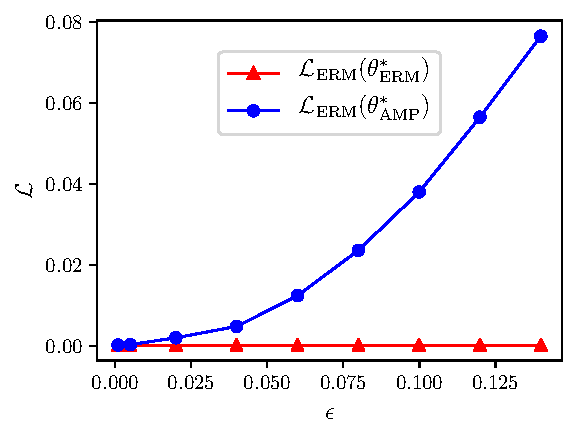
\includegraphics[width=.45\textwidth]{figs/tune_a.pdf}}
\subcaptionbox{CIFAR-10 Test Set}[.48\textwidth]{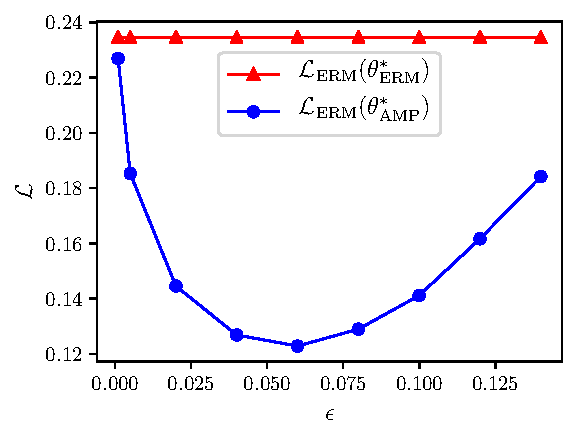
\includegraphics[width=.45\textwidth]{figs/tune_b.pdf}}
\end{figure}

\end{frame}

\begin{frame}{Flatness of the Selected Minima}
\begin{figure}
\subcaptionbox{ERM Training Loss}[.48\textwidth]{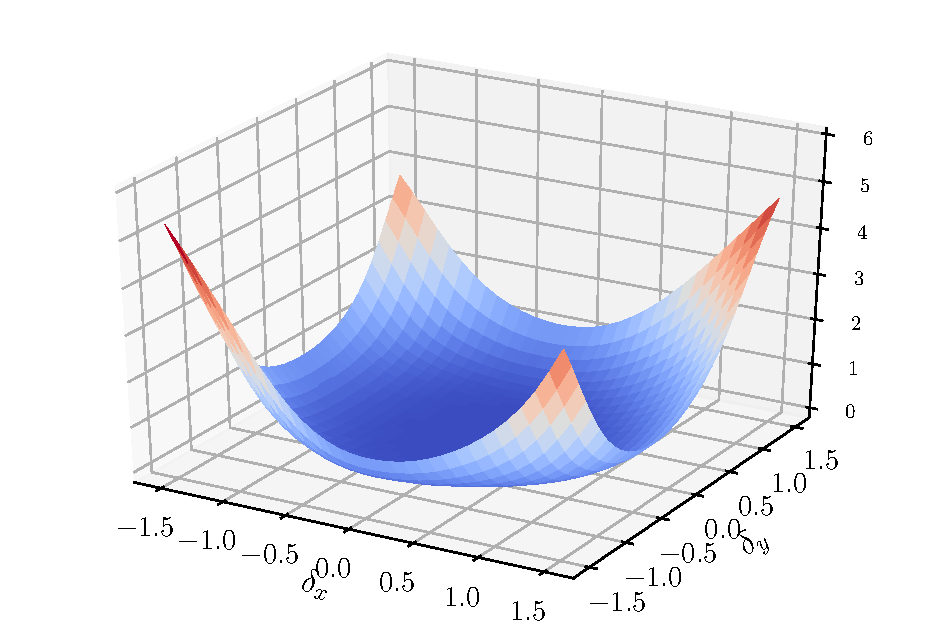
\includegraphics[width=.28\textwidth]{figs/svhn_erm_train_loss_landscape3D.pdf}}
\subcaptionbox{ERM Test Loss}[.48\textwidth]{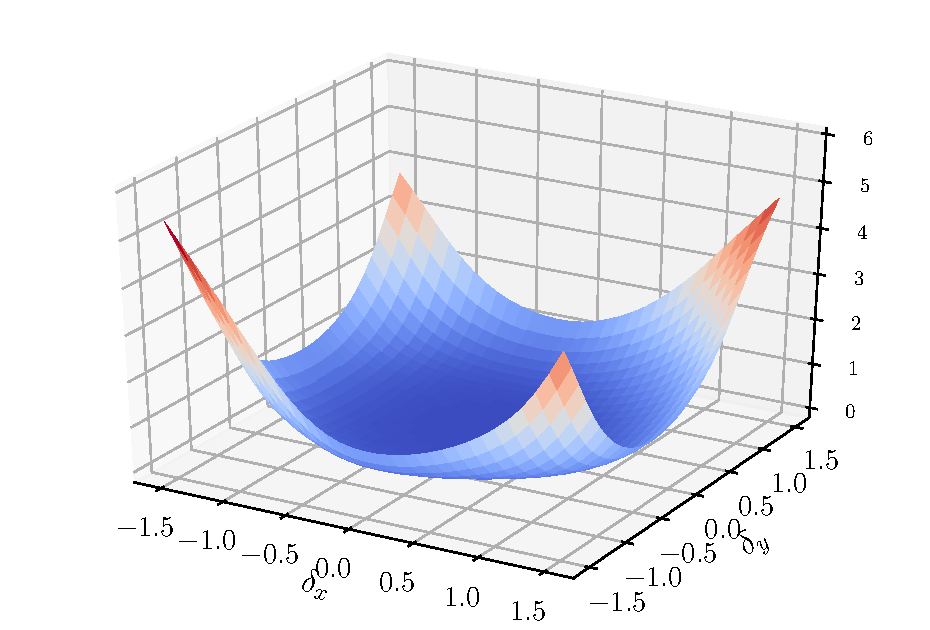
\includegraphics[width=.28\textwidth]{figs/svhn_erm_test_loss_landscape3D.pdf}}
\subcaptionbox{AMP Training Loss}[.48\textwidth]{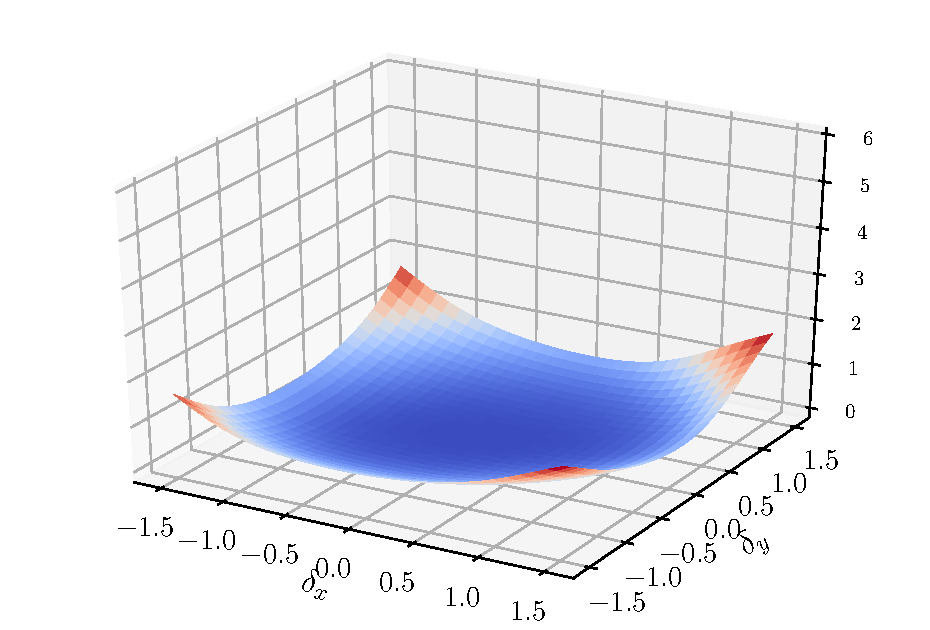
\includegraphics[width=.28\textwidth]{figs/svhn_amp_train_loss_landscape3D.pdf}}
\subcaptionbox{AMP Test Loss}[.48\textwidth]{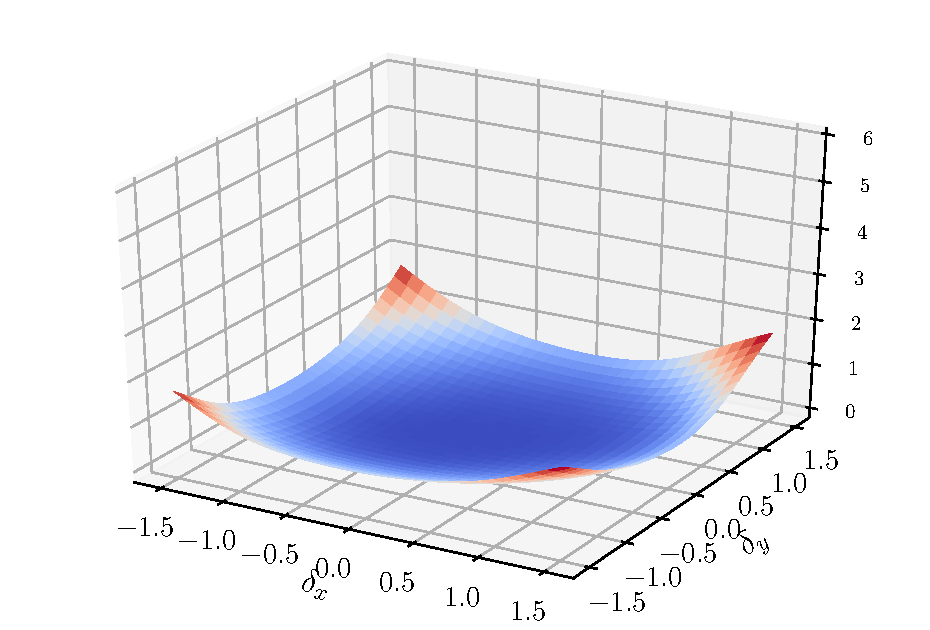
\includegraphics[width=.28\textwidth]{figs/svhn_amp_test_loss_landscape3D.pdf}}
\end{figure}
\end{frame}
